\section{Hardware Implementation}
\subsection{Microcontroller peripherals}
Before choosing which pins on the Arduino Mega to connect the various hardware to, the peripherals\footnote{Hardware modules, such as timers, UARTs, etc.} in the microcontroller needs to be evaluated (each peripheral is only available on certain pins). First, the timers are considered. The microcontroller has 6 hardware timers, \emph{Timer 0 - Timer 5}.

Timer 0 is reserved by the Arduino itself, and not to be touched. \todo{source} This leaves 5 timers, that can be used freely.

It would be advantageous to utilize the input capture\footnote{An input capture timer samples a free running counter, whenever triggered by  an external event} functionality of the timers to read the hall sensors. After examining the Arduino Mega pinout (\secref{megaPinout}), it is seen that only Timer 4 and 5 have their input capture pins available on the board (ICP4 and ICP5). These are therefore chosen for the hall sensors.
   
The realtime operating system needs a timer, for running it's scheduler. Timer 1 is chosen for this, for no other reason than it being the default setting.

This leaves Timer 2 and 3. According to the datasheet of the microcontroller, Timer 2 is an 8 bit timer, and Timer 3 is 16 bit. 

Timer 3 is chosen for the servo. This, because the higher resolution makes it easier to generate the short duty cycles required by the servo (500us to 2500us on-time, in a 30ms period, see \subsecref{Servo})

The last timer is chosen for the DC-motor.

As the timers has now been designated, the next will be the various serial ports. The XBee module needs to connect to a serial port, and UART3 is chosen, as it makes it easiest to route the PCB traces. The SD-card needs an SPI connection, and must therefore be connected to the SPI pins. Lastly, the "9 Degrees of Freedom"-board needs an $\text{I}^2\text{C}$ connection, and has to be connected to the Arduino's $\text{I}^2\text{C}$ pins.

As all hardware modules have now been assigned pins on the Arduino, the electrical requirements of each module will now be considered.

\subsection{Electrical considerations}

Before connecting hardware modules to the Arduino pins, signal voltage levels need to be considered:

\begin{itemize}
\item The Arduino itself uses 5V logic levels.
\todo{source} 
\item The "9 Degrees of Freedom"-board needs 5V supply voltage and $\SI{3,3}{V}$ logic levels
\todo{source}
\item The servo needs $\SI{4,8}{V}$ - 6V supply voltage and 5V signal levels
\todo{source}
\item The SD-card needs $\SI{3,3}{V}$ supply voltage and signal levels
\todo{source}
\item The Hall sensors need $\SI{3,5}{V}$ - 24V supply, and a pull up resistor to define the logic level.
\todo{source}
\item The XBee needs $\SI{3,3}{V}$ supply voltage and signal levels
\todo{source}
\end{itemize} 

The Arduino has regulated 5V and $\SI{3,3}{V}$ supply rails available, which will be used to power the respectable hardware modules. As the servo can potentially draw a lot of current, and overload the Arduino, it will be connected to a dedicated 5V voltage regulator, powered directly from the battery.

A low-dropout type is chosen, \textbf{L4941}, to make sure it works, even at low battery voltages. This regulator has a maximum dropout of 700mV at 1A current, meaning that it will work with battery voltages as low as $\SI{5,7}{V}$. \todo{datasheet} 

All one-directional connections from the Arduino to  $\SI{3,3}{V}$ logic level inputs will be connected to a HEF4050 CMOS buffer. This device can accept input voltages up to 15V, while supplied by as little as 3V supply voltage. This makes it ideal for uni-directional voltage level translation. \todo{datasheet}

One-directional connection from  $\SI{3,3}{V}$ logic level output to Arduino inputs will be connected directly, as $\SI{3,3}{V}$ is above the minimum high level threshold (Min $\text{V}_\text{IH}=\SI{0,6}\cdot \text{Vcc} = \SI{0,6}\cdot 5 = 3$V). \todo{source}

As the $\text{I}^2\text{C}$ bus is using bi-directional connections, and needs to connect a $\SI{3,3}{V}$ system to a 5V system, this needs to be addressed as well. One solution could be running the bus at $\SI{3,3}{V}$, but this is unfortunately not possible, as the microcontroller needs at least $\SI{3,5}{V}$ as HIGH voltage, when in  $\text{I}^2\text{C}$ mode. \todo{ref}The creators of $\text{I}^2\text{C}$, Philips, recommends solving this with two mosfets, see \figref{i2clevel}.

\begin{figure}[H]
	\centering
	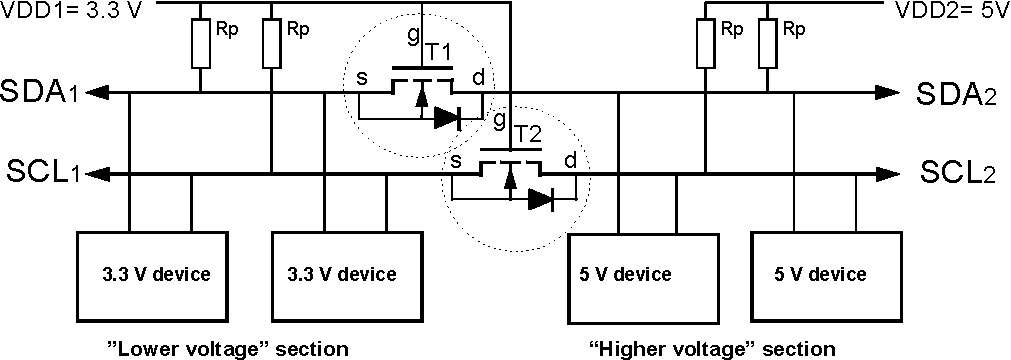
\includegraphics[scale=0.9]{figures/i2cLevel.pdf}
	\caption{$\text{I}^2\text{C}$ Voltage level translator. [source: Philips]}
	\label{i2clevel}
\end{figure}

